\documentclass[11pt, a4paper]{report}
%\documentclass[11pt, a4paper]{article}

%====================== PACKAGES ======================


\usepackage[french]{babel}

\frenchbsetup{StandardLists=true}
\usepackage{enumitem}
\usepackage{pifont}

\usepackage[utf8x]{inputenc}
%\usepackage[latin1]{inputenc} % Feynman

%pour gérer les positionnement d'images
\usepackage{float}
\usepackage{amsmath}
\DeclareMathOperator{\dt}{dt}
\usepackage{graphicx}
\usepackage{tabularx}
\usepackage[colorinlistoftodos]{todonotes}
\usepackage{url}
%pour les informations sur un document compilé en PDF et les liens externes / internes
\usepackage[pdfborder=0]{hyperref}
\hypersetup{
	colorlinks = true
	}
%pour la mise en page des tableaux
\usepackage{array}
\usepackage{tabularx}
\usepackage{multirow}
\usepackage{multicol}
\setlength{\columnsep}{50pt}
%pour utiliser \floatbarrier
%\usepackage{placeins}
%\usepackage{floatrow}
%espacement entre les lignes
\usepackage{setspace}
%modifier la mise en page de l'abstract
\usepackage{abstract}
%police et mise en page (marges) du document
\usepackage[T1]{fontenc}
\usepackage[top=2cm, bottom=2cm, left=2cm, right=2cm]{geometry}
%Pour les galerie d'images
\usepackage{subfig}

\usepackage{pdfpages}
\usepackage{tikz}
%\usepackage{tikz}
\usetikzlibrary{trees}
\usetikzlibrary{decorations.pathmorphing}
\usetikzlibrary{decorations.markings}
\usetikzlibrary{decorations.pathreplacing,calligraphy}
\usetikzlibrary{decorations.pathmorphing,calc,shapes,shapes.geometric,patterns}
%\usetikzlibrary{decorations}
\usetikzlibrary{angles, quotes}
\usepackage{verbatim}

\usepackage{appendix}

\usepackage{comment}

\usepackage{xcolor}

\hypersetup{colorlinks=true,linkcolor=black}

\usepackage{makeidx}

%\PreviewEnvironment{tikzpicture}
%\setlength\PreviewBorder{0pt}%

%====================== INFORMATION ET REGLES ======================

%rajouter les numérotation pour les \paragraphe et \subparagraphe
\setcounter{secnumdepth}{4}
\setcounter{tocdepth}{4}

\hypersetup{							% Information sur le document
pdfauthor = {Stephan Runigo},			% Auteurs
pdftitle = {Documentation},			% Titre du document
pdfsubject = {Documentation},		% Sujet
pdfkeywords = {Document},	% Mots-clefs
pdfstartview={FitH}}	% ajuste la page à la largeur de l'écran
%pdfcreator = {MikTeX},% Logiciel qui a crée le document
%pdfproducer = {} % Société avec produit le logiciel
\makeindex % Créer un index
%======================== DEBUT DU DOCUMENT ========================
%
\begin{document}
%
%régler l'espacement entre les lignes
\newcommand{\HRule}{\rule{\linewidth}{0.5mm}}
%
% Titre, résumé, ... %
%
\begin{titlepage}
%
~\\[1cm]

\begin{center}
%\includegraphics[scale=0.5]{./presentation/chambreABulle}
\end{center}

\textsc{\Large }\\[0.5cm]

% Title \\[0.4cm]
\HRule

\begin{center}
{\huge \bfseries  La causalité\\
%titre 2\\[0.4cm]
 }
\end{center}

\HRule \\[1.5cm]

\begin{center}
%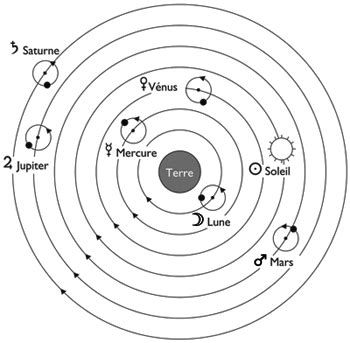
\includegraphics[scale=0.3]{./presentation/ptoleme}
\end{center}

\begin{center}
%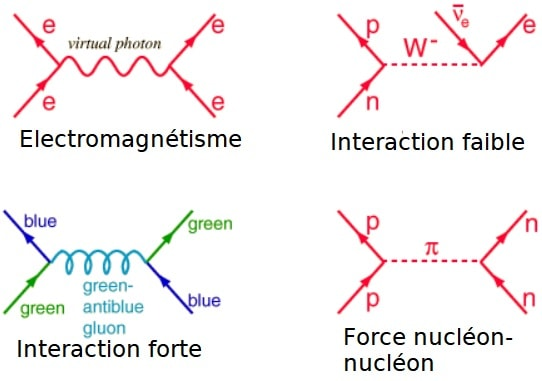
\includegraphics[scale=0.3]{./presentation/diagrammesInteractions}
\end{center}


% Author and supervisor
\begin{minipage}{0.4\textwidth}
\begin{flushleft} \large
%\emph{Auteur:}\\
%Stephan \textsc{Runigo}
\end{flushleft}
\end{minipage}
\begin{minipage}{0.4\textwidth}
\begin{flushright} \large
\emph{Auteur:}\\
Stephan \textsc{Runigo}
\end{flushright}
\end{minipage}

\vfill

% Bottom of the page
{\large \today}

\end{titlepage}

\newpage
\begin{center}
\Large
Résumé
\normalsize
\end{center}
\vspace{3cm}
\begin{itemize}[leftmargin=1cm, label=\ding{32}, itemsep=21pt]
\item {\bf Objet : } Souvenir des questions posés.
\item {\bf Contenu : } Définition, analyse, reflexion.
\item {\bf Public concerné : } Interressé à la question de l'âme.
\end{itemize}

\vspace{3cm}



\vspace{3cm}


%

%
% Table des matières
\tableofcontents
\thispagestyle{empty}
\setcounter{page}{0}
%
%espacement entre les lignes des tableaux
\renewcommand{\arraystretch}{1.5}
%
%====================== INCLUSION DES CHAPITRES ======================
%
~
\thispagestyle{empty}
%recommencer la numérotation des pages à "1"
\setcounter{page}{0}
\newpage
%
%\chapter{Énergie}
%

%%%%%%%%%%%%%%%%%%%%%
\section{Chute libre}
%%%%%%%%%%%%%%%%%%%%%
%
%\subsection{Définition}

On lache une balle. On observe que celle-ci se met en mouvement, se dirige vers le bas, puis frappe le sol. Cette succession d'évènements constitue un phénomène : le phénomène de la chute libre.
\begin{center}

%%%%%%%%%%%%%%%%%%%%%        PERSONNAGE AU BORD D'UNE MARE
%  DÉFINITIONS

\tikzset{
  feuillage/.style = {decoration={random steps, segment length=0.4mm}, decorate},
  tronc/.style   = {decoration={random steps, segment length=2mm, amplitude=0.2mm}, decorate}}

\tikzset{  arbre/.pic={ \foreach \w/\f in {0.3/30,0.2/50,0.1/70} { \fill [brown!\f!black, tronc] (-\w/2,0) rectangle +(\w,3); } \foreach \n/\f in {1.4/40,1.2/50,1/60,0.8/70,0.6/80,0.4/90} { \fill [green!\f!black, feuillage](0,3) ellipse (\n/1.5 and \n); }}}

\tikzset{  personnage/.pic={ { \fill [black] (0,0)ellipse(0.25 and 0.55); } 
  { \fill [black](0,0.75)circle(0.2); }
    % jambe et pieds
  {\fill [rounded corners=2pt] (0.1,-0.3)rectangle(-0.1,-1.5);}
  {\fill [rounded corners=2pt] (0.3,-1.4)rectangle(-0.1,-1.5);}
    % bras
  {\fill [rounded corners=2pt, rotate=-15] (-0.1,0.42)rectangle(0.5,0.29);}
  {\fill [rounded corners=2pt] (0.44,0.17)rectangle(1,0.29);}}}

\begin{tikzpicture}%[scale=0.5]
    %  Ciel
  \shade[bottom color=cyan!60!black, top color=blue!20!white] (0,0) rectangle (7.5,2.2);
    %  Sol
  \shade[bottom color=green!50!black, top color=green!70!black] (0,0.5) rectangle (7.5,-1);
    %  Mare
 % \shade[bottom color=blue!50!white, top color=cyan!60!black] (3.7,-0.15) ellipse (2.5 and 0.3);
    %  Arbre
 % \pic at (2,2)    {arbre};

    %  Personnage
  \begin{scope}[xshift=1 cm,yshift=0.6 cm]
    % corps et tête
 \fill [black] (0,0)ellipse(0.12 and 0.27);
 \fill [black](0,0.37)circle(0.1);
    % jambe et pieds
 \fill [rounded corners=2pt] (0.05,-0.15)rectangle(-0.05,-0.75);
 \fill [rounded corners=2pt] (0.15,-0.7)rectangle(-0.05,-0.75);
    % bras
 \fill [rounded corners=2pt, rotate=-15] (-0.1,0.22)rectangle(0.28,0.15);
 \fill [rounded corners=2pt] (0.22,0.08)rectangle(0.5,0.14);
   % Balle
 \fill[red] (0.5,0.05) circle(0.05);
  \end{scope}

\end{tikzpicture}

%%%%%%%%%%%%%%%%%%%%%%%%%%%%%%%%%%%%%%%%%%%%%%%%%%%%%%%%%%%%%%%%%%%%%%%%%%%%%%%%

\end{center}

%\subsection{Paradigmes}

Il existe plusieurs paradigmes qui tente de donner une explication rationnelle à ce phénomène. Pour aristote, la balle constituée de matière terrestre souhaite rejoindre le lieu de la matière terrestre qui est le bas. Pour Newton, la force gravitationnelle entre la Terre et la balle provoque la mise en mouvement de la balle. Pour Lagrange et Hamilton, l'énergie potentielle de gravitation de la balle se convertie en énergie cinétique. 


L'énergie potentielle est relié à la position, l'énergie cinétique est relié au mouvement, à la vitesse.

%\begin{minipage}[c]{.45\linewidth}
\begin{center}
Vision "Force de Gravitation"
\end{center}
La Terre exerce une force de gravitation $\overrightarrow{F}_{T/B}$ sur la balle $B$
%\setlength{\unitlength}{1cm}
\begin{center}
%
%%%%%%%%%%%%%%%%%%%%%        PERSONNAGE AU BORD D'UNE MARE
%  DÉFINITIONS

\tikzset{
  feuillage/.style = {decoration={random steps, segment length=0.4mm}, decorate},
  tronc/.style   = {decoration={random steps, segment length=2mm, amplitude=0.2mm}, decorate}}

\tikzset{  arbre/.pic={ \foreach \w/\f in {0.3/30,0.2/50,0.1/70} { \fill [brown!\f!black, tronc] (-\w/2,0) rectangle +(\w,3); } \foreach \n/\f in {1.4/40,1.2/50,1/60,0.8/70,0.6/80,0.4/90} { \fill [green!\f!black, feuillage](0,3) ellipse (\n/1.5 and \n); }}}

\tikzset{  personnage/.pic={ { \fill [black] (0,0)ellipse(0.25 and 0.55); } 
  { \fill [black](0,0.75)circle(0.2); }
    % jambe et pieds
  {\fill [rounded corners=2pt] (0.1,-0.3)rectangle(-0.1,-1.5);}
  {\fill [rounded corners=2pt] (0.3,-1.4)rectangle(-0.1,-1.5);}
    % bras
  {\fill [rounded corners=2pt, rotate=-15] (-0.1,0.42)rectangle(0.5,0.29);}
  {\fill [rounded corners=2pt] (0.44,0.17)rectangle(1,0.29);}}}

\begin{tikzpicture}%[scale=0.5]
    %  Ciel
  \shade[bottom color=cyan!60!black, top color=blue!20!white] (0,0) rectangle (7.5,2.2);
    %  Sol
  \shade[bottom color=green!50!black, top color=green!70!black] (0,0.5) rectangle (7.5,-1);
    %  Mare
 % \shade[bottom color=blue!50!white, top color=cyan!60!black] (3.7,-0.15) ellipse (2.5 and 0.3);
    %  Arbre
 % \pic at (2,2)    {arbre};

    %  Personnage
  \begin{scope}[xshift=1 cm,yshift=0.6 cm]
    % corps et tête
 \fill [black] (0,0)ellipse(0.12 and 0.27);
 \fill [black](0,0.37)circle(0.1);
    % jambe et pieds
 \fill [rounded corners=2pt] (0.05,-0.15)rectangle(-0.05,-0.75);
 \fill [rounded corners=2pt] (0.15,-0.7)rectangle(-0.05,-0.75);
    % bras
 \fill [rounded corners=2pt, rotate=-15] (-0.1,0.22)rectangle(0.28,0.15);
 \fill [rounded corners=2pt] (0.22,0.08)rectangle(0.5,0.14);
   % Balle
 \fill[red] (0.5,0.05) circle(0.05);
  \end{scope}

\end{tikzpicture}

%%%%%%%%%%%%%%%%%%%%%%%%%%%%%%%%%%%%%%%%%%%%%%%%%%%%%%%%%%%%%%%%%%%%%%%%%%%%%%%%

\texttt{FIGURE}
\end{center}
%\end{minipage}
%\hfill
%\begin{minipage}[c]{.45\linewidth}
\begin{center}
Vision "Énergétique"
\end{center}
La balle possède une énergie potentielle de gravitation lié à son altitude, au cours de sa chute, elle acquiert une énergie cinétique lié à sa vitesse. Au cours de la chutte, l'énergie potentielle est convertie en énergie cinétique. L'énergie totale, reste constante.
\begin{center}
%
%%%%%%%%%%%%%%%%%%%%%        PERSONNAGE AU BORD D'UNE MARE
%  DÉFINITIONS

\tikzset{
  feuillage/.style = {decoration={random steps, segment length=0.4mm}, decorate},
  tronc/.style   = {decoration={random steps, segment length=2mm, amplitude=0.2mm}, decorate}}

\tikzset{  arbre/.pic={ \foreach \w/\f in {0.3/30,0.2/50,0.1/70} { \fill [brown!\f!black, tronc] (-\w/2,0) rectangle +(\w,3); } \foreach \n/\f in {1.4/40,1.2/50,1/60,0.8/70,0.6/80,0.4/90} { \fill [green!\f!black, feuillage](0,3) ellipse (\n/1.5 and \n); }}}

\tikzset{  personnage/.pic={ { \fill [black] (0,0)ellipse(0.25 and 0.55); } 
  { \fill [black](0,0.75)circle(0.2); }
    % jambe et pieds
  {\fill [rounded corners=2pt] (0.1,-0.3)rectangle(-0.1,-1.5);}
  {\fill [rounded corners=2pt] (0.3,-1.4)rectangle(-0.1,-1.5);}
    % bras
  {\fill [rounded corners=2pt, rotate=-15] (-0.1,0.42)rectangle(0.5,0.29);}
  {\fill [rounded corners=2pt] (0.44,0.17)rectangle(1,0.29);}}}

\begin{tikzpicture}%[scale=0.5]
    %  Ciel
  \shade[bottom color=cyan!60!black, top color=blue!20!white] (0,0) rectangle (7.5,2.2);
    %  Sol
  \shade[bottom color=green!50!black, top color=green!70!black] (0,0.5) rectangle (7.5,-1);
    %  Mare
 % \shade[bottom color=blue!50!white, top color=cyan!60!black] (3.7,-0.15) ellipse (2.5 and 0.3);
    %  Arbre
 % \pic at (2,2)    {arbre};

    %  Personnage
  \begin{scope}[xshift=1 cm,yshift=0.6 cm]
    % corps et tête
 \fill [black] (0,0)ellipse(0.12 and 0.27);
 \fill [black](0,0.37)circle(0.1);
    % jambe et pieds
 \fill [rounded corners=2pt] (0.05,-0.15)rectangle(-0.05,-0.75);
 \fill [rounded corners=2pt] (0.15,-0.7)rectangle(-0.05,-0.75);
    % bras
 \fill [rounded corners=2pt, rotate=-15] (-0.1,0.22)rectangle(0.28,0.15);
 \fill [rounded corners=2pt] (0.22,0.08)rectangle(0.5,0.14);
   % Balle
 \fill[red] (0.5,0.05) circle(0.05);
  \end{scope}

\end{tikzpicture}

%%%%%%%%%%%%%%%%%%%%%%%%%%%%%%%%%%%%%%%%%%%%%%%%%%%%%%%%%%%%%%%%%%%%%%%%%%%%%%%%

\texttt{FIGURE}
\end{center}
%Le champ électrique $\overrightarrow{E}$ exerce une force $\overrightarrow{F}_{\overrightarrow{E}/Q_2}$ sur la charge électrique $Q_2$
%\end{minipage}

%\subsection{Champ magnétique}

%%%%%%%%%%%%%%%%%%%%%%%%%%%%%%%%%%%%%%%%%%%%%%%%%%%%%%%%%%%%%%%%%%%%%%%%%%%%

%

%%%%%%%%%%%%%%%%%%%%%
\section{Pendule simple}
%%%%%%%%%%%%%%%%%%%%%
%
%\subsection{Définition}

%Un champ est la donnée de sa valeur en tout point de l'espace. Cette valeur peut être scalaire ou vectoriel. Elle peut éventuellement être variable au cours du temps, elle est généralement variable dans l'espace.

\subsection{Définition}

Un pendule simple est une masse suspendue à une tige rigide pouvant pivoter en un point. Un tel dispositif possède une position d'équilibre, et un mouvement oscillatoir autour de cette position.



%%%%%%%%%%%%%%%%%%%%%
\section{Oscillateur harmonique}
%%%%%%%%%%%%%%%%%%%%%

\begin{center}
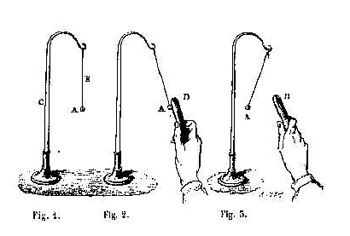
\includegraphics[scale=0.9]{./theorieDesChamps/MascartTraiteDElectriciteStatique1876}
\end{center}

\begin{minipage}[c]{.45\linewidth}
\begin{center}
Vision "Force de Coulomb"
\end{center}
Une charge électrique $Q_1$ exerce une force de Coulomb $\overrightarrow{F}_{Q_1/Q_2}$ sur la charge électrique $Q_2$
\setlength{\unitlength}{1cm}
\begin{picture}(10,3)
\put(0.5,1.0){\circle{0.3}}
\put(0.3,0.3){$Q_1$}
%\put(0.5,1.0){\vector(1,0){1.36}}
%\put(1.2,1.3){$\overrightarrow{F}_{Q_2/Q_1}$}
\put(5.5,1.0){\circle{0.5}}
\put(5.3,0.2){$Q_2$}
\put(5.5,1.0){\vector(-1,0){1.36}}
\put(3.7,1.3){$\overrightarrow{F}_{Q_1/Q_2}$}
\end{picture}
%On peut alors se demander comment l'information de la présence de $Q_1$ parvient à $Q_2$, y a-t-il quelque chose qui se propage entre les charges ? Cette question peut être simplifiée en disant que les charges créent un champ dans tout l'espace et qu'elle sont sensibles à ce champ.
\end{minipage}
\hfill
\begin{minipage}[c]{.45\linewidth}
\begin{center}
Vision "Champ électrique"
\end{center}
Une charge électrique $Q_1$ crée un champ électrique $\overrightarrow{E}$ dans tout l'espace.
\setlength{\unitlength}{1cm}
\begin{picture}(10,3)
\put(0.5,1.0){\circle{0.3}}
\put(0.3,0.3){$Q_1$}
\put(5.5,1.0){\vector(-1,0){1.36}}
\put(3.7,1.3){$\overrightarrow{E}$}
\end{picture}
Le champ électrique $\overrightarrow{E}$ exerce une force $\overrightarrow{F}_{\overrightarrow{E}/Q_2}$ sur la charge électrique $Q_2$
\setlength{\unitlength}{1cm}
\begin{picture}(10,3)
\put(5.5,1.0){\circle{0.5}}
\put(5.3,0.2){$Q_2$}
\put(5.5,1.0){\vector(-1,0){1.36}}
\put(3.7,1.3){$\overrightarrow{F}_{\overrightarrow{E}/Q_2}$}
\end{picture}
\end{minipage}

Le champ créé par une charge électrique est à priori un outil purement mathématique, un artifice de calcul bien pratique. L'existence de ce "champ électrique" est à priori hypothétique. Néanmoins, son existence permet d'interpréter la transmission de "l'information de présence" entre les charges, de lever l'hypothèse d'une transmission d'information instantanée et immatérielle entre les charges.

\subsection{Champ magnétique}

De la même façon que pour l'électrostatique, les physiciens vont introduire le champs magnétique afin de "nommer à priori" le "médiateur" entre les aimants "expliquant" leurs interactions.

\subsection{Autres exemples de champs}

Champ de température dans l'atmosphère terrestre, champ d'altitude sur une carte topographique.

%%%%%%%%%%%%%%%%%%%%%%%%%%%%%%%%%%%%%%%%%%%%%%%%%%%%%%%%%%%%%%%%%%%%%%%%%%%%

%
%

%
\chapter{Théorie des champs}
%
%
%%%%%%%%%%%%%%%%%%%%%
\section{Force électrostatique}
%%%%%%%%%%%%%%%%%%%%%
%

Les forces électrostatiques s'exerçent entre les particules chargées. Les charges électriques peuvent être positive ou négative.
%La loi de Coulomb indique que des corps chargés électriquement exercent entre eux des forces. 
Des charges électriques de même signe se repousent, des charges de signe opposées s'attirent.

%
Un batonnet en matière synthétique (règle en plastique) frottée à l'aide d'un chiffon, s'électrise. Il est alors capable d'attirer des petits bouts de papier.

\begin{center}
\texttt{FIGURE}
\end{center}

% Lors du frottements, des électrons sont arraché à la matière et s'accumulent sur l'un 
 Dans l'expérience du pendule électrostatique, le batonnet attire le pendule (constitué d'une petite boule de papier aluminium).
% (le pendule n'est pas chargé mais la force de Coulomb crée une polarisation),
Lorsque le pendule touche le batonnet, un transfert de charge a lieu, le pendule se charge électriquement, et est alors repoussé.

\begin{center}
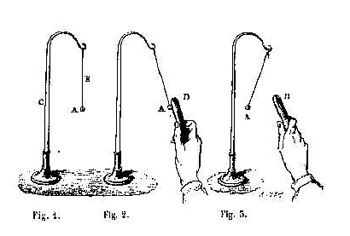
\includegraphics[scale=0.9]{./theorieDesChamps/MascartTraiteDElectriciteStatique1876}
\end{center}

L'expérience du pendule électrostatique peut se modéliser par des {\it forces électrostatiques} s'exerçant entre les particules chargées. Ce modèle suppose une {\it action à distance}.

% Dans un second temps, elle peut se modéliser par  en disant qu'une particule chargée crée un champ électrostatique en tout point de l'espace et qu'une particule chargée placé dans un champ électrostatique subit une force.

%\begin{minipage}[c]{.45\linewidth}
\begin{center}
Vision "Force de Coulomb"
\end{center}
Une charge électrique $Q_1$ exerce une force de Coulomb $\overrightarrow{F}_{Q_1/Q_2}$ sur la charge électrique $Q_2$

\begin{center}
\setlength{\unitlength}{1cm}
\begin{picture}(10,3)
\put(0.5,1.0){\circle{0.3}}
\put(0.3,0.3){$Q_1$}
%\put(0.5,1.0){\vector(1,0){1.36}}
%\put(1.2,1.3){$\overrightarrow{F}_{Q_2/Q_1}$}
\put(5.5,1.0){\circle{0.5}}
\put(5.3,0.2){$Q_2$}
\put(5.5,1.0){\vector(-1,0){1.36}}
\put(3.7,1.3){$\overrightarrow{F}_{Q_1/Q_2}$}
\end{picture}
\end{center}
%On peut alors se demander comment l'information de la présence de $Q_1$ parvient à $Q_2$, y a-t-il quelque chose qui se propage entre les charges ? Cette question peut être simplifiée en disant que les charges créent un champ dans tout l'espace et qu'elle sont sensibles à ce champ.
%\end{minipage}\hfill\begin{minipage}[c]{.45\linewidth}

%%%%%%%%%%%%%%%%%%%%%%%%%%%%%%%%%%%%%%%%%%%%%%%%%%%%%%%%%%%%%%%%%%%%%%%%%%%%

%
%
%%%%%%%%%%%%%%%%%%%%%
\section{Champ électrostatique}
%%%%%%%%%%%%%%%%%%%%%
%
%\subsection{Définition}
L'expérience du pendule électrostatique peut se modéliser par des {\it forces électrostatiques} s'exerçant entre les particules chargées. Ce modèle suppose une {\it action à distance}. La notion de champs permet de modéliser cette action entre les charges électriques : une charge électrique crée un champ dans tout l'espace. Le champ exercent une force sur les charges électriques.

\begin{center}
Vision "Champ électrique"
\end{center}
Une charge électrique $Q_1$ crée un champ électrique $\overrightarrow{E}$ dans tout l'espace.

\begin{center}
\setlength{\unitlength}{1cm}
\begin{picture}(10,3)
\put(0.5,1.0){\circle{0.3}}
\put(0.3,0.3){$Q_1$}
\put(5.5,1.0){\vector(-1,0){1.36}}
\put(3.7,1.3){$\overrightarrow{E}$}
\end{picture}
\end{center}

Le champ électrique $\overrightarrow{E}$ exerce une force $\overrightarrow{F}_{\overrightarrow{E}/Q_2}$ sur la charge électrique $Q_2$

\setlength{\unitlength}{1cm}
\begin{picture}(10,3)
\put(5.5,1.0){\circle{0.5}}
\put(5.3,0.2){$Q_2$}
\put(5.5,1.0){\vector(-1,0){1.36}}
\put(3.7,1.3){$\overrightarrow{F}_{\overrightarrow{E}/Q_2}$}
\end{picture}

Le champ créé par une charge électrique est à priori un outil purement mathématique, un artifice de calcul bien pratique. L'existence de ce "champ électrique" est à priori hypothétique. Néanmoins, son existence permet d'interpréter la transmission de "l'information de présence" entre les charges, de lever l'hypothèse d'une transmission d'information instantanée et immatérielle entre les charges.

%%%%%%%%%%%%%%%%%%%%%%%%%%%%%%%%%%%%%%%%%%%%%%%%%%%%%%%%%%%%%%%%%%%%%%%%%%%%

%
%
%%%%%%%%%%%%%%%%%%%%%
\section{Champ magnétique}
%%%%%%%%%%%%%%%%%%%%%
%
Les aimants exercent entre eux des forces magnétiques.

\begin{center}
%
%%%%%%%%%%%%%%%%%%%%%        PERSONNAGE AU BORD D'UNE MARE
%  DÉFINITIONS

\tikzset{
  feuillage/.style = {decoration={random steps, segment length=0.4mm}, decorate},
  tronc/.style   = {decoration={random steps, segment length=2mm, amplitude=0.2mm}, decorate}}

\tikzset{  arbre/.pic={ \foreach \w/\f in {0.3/30,0.2/50,0.1/70} { \fill [brown!\f!black, tronc] (-\w/2,0) rectangle +(\w,3); } \foreach \n/\f in {1.4/40,1.2/50,1/60,0.8/70,0.6/80,0.4/90} { \fill [green!\f!black, feuillage](0,3) ellipse (\n/1.5 and \n); }}}

\tikzset{  personnage/.pic={ { \fill [black] (0,0)ellipse(0.25 and 0.55); } 
  { \fill [black](0,0.75)circle(0.2); }
    % jambe et pieds
  {\fill [rounded corners=2pt] (0.1,-0.3)rectangle(-0.1,-1.5);}
  {\fill [rounded corners=2pt] (0.3,-1.4)rectangle(-0.1,-1.5);}
    % bras
  {\fill [rounded corners=2pt, rotate=-15] (-0.1,0.42)rectangle(0.5,0.29);}
  {\fill [rounded corners=2pt] (0.44,0.17)rectangle(1,0.29);}}}

\begin{tikzpicture}%[scale=0.5]
    %  Ciel
  \shade[bottom color=cyan!60!black, top color=blue!20!white] (0,0) rectangle (7.5,2.2);
    %  Sol
  \shade[bottom color=green!50!black, top color=green!70!black] (0,0.5) rectangle (7.5,-1);
    %  Mare
 % \shade[bottom color=blue!50!white, top color=cyan!60!black] (3.7,-0.15) ellipse (2.5 and 0.3);
    %  Arbre
 % \pic at (2,2)    {arbre};

    %  Personnage
  \begin{scope}[xshift=1 cm,yshift=0.6 cm]
    % corps et tête
 \fill [black] (0,0)ellipse(0.12 and 0.27);
 \fill [black](0,0.37)circle(0.1);
    % jambe et pieds
 \fill [rounded corners=2pt] (0.05,-0.15)rectangle(-0.05,-0.75);
 \fill [rounded corners=2pt] (0.15,-0.7)rectangle(-0.05,-0.75);
    % bras
 \fill [rounded corners=2pt, rotate=-15] (-0.1,0.22)rectangle(0.28,0.15);
 \fill [rounded corners=2pt] (0.22,0.08)rectangle(0.5,0.14);
   % Balle
 \fill[red] (0.5,0.05) circle(0.05);
  \end{scope}

\end{tikzpicture}

%%%%%%%%%%%%%%%%%%%%%%%%%%%%%%%%%%%%%%%%%%%%%%%%%%%%%%%%%%%%%%%%%%%%%%%%%%%%%%%%

\texttt{FIGURE : aimants, bousole}
\end{center}

De la même façon que pour l'électrostatique, les physiciens vont introduire le champ magnétique afin de "nommer à priori" le "médiateur" entre les aimants "expliquant" leurs interactions.

\begin{center}
%
%%%%%%%%%%%%%%%%%%%%%        PERSONNAGE AU BORD D'UNE MARE
%  DÉFINITIONS

\tikzset{
  feuillage/.style = {decoration={random steps, segment length=0.4mm}, decorate},
  tronc/.style   = {decoration={random steps, segment length=2mm, amplitude=0.2mm}, decorate}}

\tikzset{  arbre/.pic={ \foreach \w/\f in {0.3/30,0.2/50,0.1/70} { \fill [brown!\f!black, tronc] (-\w/2,0) rectangle +(\w,3); } \foreach \n/\f in {1.4/40,1.2/50,1/60,0.8/70,0.6/80,0.4/90} { \fill [green!\f!black, feuillage](0,3) ellipse (\n/1.5 and \n); }}}

\tikzset{  personnage/.pic={ { \fill [black] (0,0)ellipse(0.25 and 0.55); } 
  { \fill [black](0,0.75)circle(0.2); }
    % jambe et pieds
  {\fill [rounded corners=2pt] (0.1,-0.3)rectangle(-0.1,-1.5);}
  {\fill [rounded corners=2pt] (0.3,-1.4)rectangle(-0.1,-1.5);}
    % bras
  {\fill [rounded corners=2pt, rotate=-15] (-0.1,0.42)rectangle(0.5,0.29);}
  {\fill [rounded corners=2pt] (0.44,0.17)rectangle(1,0.29);}}}

\begin{tikzpicture}%[scale=0.5]
    %  Ciel
  \shade[bottom color=cyan!60!black, top color=blue!20!white] (0,0) rectangle (7.5,2.2);
    %  Sol
  \shade[bottom color=green!50!black, top color=green!70!black] (0,0.5) rectangle (7.5,-1);
    %  Mare
 % \shade[bottom color=blue!50!white, top color=cyan!60!black] (3.7,-0.15) ellipse (2.5 and 0.3);
    %  Arbre
 % \pic at (2,2)    {arbre};

    %  Personnage
  \begin{scope}[xshift=1 cm,yshift=0.6 cm]
    % corps et tête
 \fill [black] (0,0)ellipse(0.12 and 0.27);
 \fill [black](0,0.37)circle(0.1);
    % jambe et pieds
 \fill [rounded corners=2pt] (0.05,-0.15)rectangle(-0.05,-0.75);
 \fill [rounded corners=2pt] (0.15,-0.7)rectangle(-0.05,-0.75);
    % bras
 \fill [rounded corners=2pt, rotate=-15] (-0.1,0.22)rectangle(0.28,0.15);
 \fill [rounded corners=2pt] (0.22,0.08)rectangle(0.5,0.14);
   % Balle
 \fill[red] (0.5,0.05) circle(0.05);
  \end{scope}

\end{tikzpicture}

%%%%%%%%%%%%%%%%%%%%%%%%%%%%%%%%%%%%%%%%%%%%%%%%%%%%%%%%%%%%%%%%%%%%%%%%%%%%%%%%

\texttt{FIGURE : ligne de champ}
\end{center}
%%%%%%%%%%%%%%%%%%%%%%%%%%%%%%%%%%%%%%%%%%%%%%%%%%%%%%%%%%%%%%%%%%%%%%%%%%%%

%
%
%%%%%%%%%%%%%%%%%%%%%
\section{Champ gravitationnel}
%%%%%%%%%%%%%%%%%%%%%
%
%\subsection{Définition}

De la même façon que l'on définit le champ électrostatique, on définit le champ gravitationnel.

%Un champ est la donnée de sa valeur en tout point de l'espace. Cette valeur peut être scalaire ou vectoriel. Elle peut éventuellement être variable au cours du temps, elle est généralement variable dans l'espace.

%%%%%%%%%%%%%%%%%%%%%%%%%%%%%%%%%%%%%%%%%%%%%%%%%%%%%%%%%%%%%%%%%%%%%%%%%%%%

%

%%%%%%%%%%%%%%%%%%%%%
%\section{Propriétés des ondes électromagnétique}
\section{Ondes électromagnétiques}
%%%%%%%%%%%%%%%%%%%%%

\subsection{Champ électrique et champ magnétique}

Au début du XIX$^\text{ème}$ siècle, les expériences de Hans Christian Oersted montrent un lien intime entre les forces magnétiques et les forces électriques : les 

Les équations de maxwell vont établir un lien entre les champs magnétique et électrique : non seuleument ces champs sont créés par les charges électrique, les aimants et les charges en mouvement, mais un champ électrique est créé par un champ magnétique variable au cours du temps et un champ magnétique est créé par un champ électrique variable au cours du temps.

%\begin{center}
\[
\overrightarrow{E} \text{ variable au cours du temps } \Rightarrow \text{ création de } \overrightarrow{B}
\]
\[
\overrightarrow{B} \text{ variable au cours du temps } \Rightarrow \text{ création de } \overrightarrow{E}
\]
%\end{center}

%\vspace{0.2cm}

\subsection{Ondes électromagnétiques et lumière}

De ces dernières propriétés découlent l'existence d'ondes électromagnétiques dont la vitesse peut être calculée en fonction des constantes électriques et magnétiques apparaissant dans les équations de Maxwell. La valeur calculée, correspondant à la valeur de la vitesse de la lumière alors connue à l'époque.

Ces ondes se propage dans le vide et dans les milieux transparent.Leur identification avec la lumière achèvera l'unification des phénomènes électriques, magnétiques et lumineux.

%%%%%%%%%%%%%%%%%%%%%%%%%%%%%%%%%%%%%%%%%%%%%%%%%%%%%%%%%%%%%%%%%%%%%%%%%%%%%

%
%

%
%
%
%====================== INCLUSION DES ANNEXES ======================
%
%%
\begin{appendix}
%

%%%%%%%%%%%%%%%%%%%%%
\chapter{Glossaire}
%%%%%%%%%%%%%%%%%%%%%

\begin{itemize}[leftmargin=1cm, label=\ding{32}, itemsep=2pt]
\item {\bf application} : en mathématique, synonyme de fonction.
\item {\bf } :
\item {\bf } :
\item {\bf quanton} : particule élémentaire satisfaisant à l'équation de schrödinger.
\item {\bf } :
\item {\bf } :
\item {\bf } :
\end{itemize}


%%%%%%%%%%%%%%%%%%%%%%%%%%%%%%%%%%%%%%%%%%%%%%%%%%%%%%%%%%%%%%%%%%%%%%%%%%%%%%%%%%%%%

%

%%%%%%%%%%%%%%%%%%%%%
\chapter{Espace vectoriel}
%%%%%%%%%%%%%%%%%%%%%

%%%%%%%%%%%%%%%%%%%%%%%%%
\section{Ensemble et application}
%%%%%%%%%%%%%%%%%%%%%%%%%
%$\mathcal{}$
Un ensemble est une collection d'objets. Ces objets sont appelés éléments (a) de l'ensemble ($\mathcal{A}$) :
\[
 a \in \mathcal{A}
\]


Une application ($f$) met en relation chaque élément ($a$) d'un ensemble ($\mathcal{A}$, dit de départ) avec un élément ($b$) d'un autre ensemble ($\mathcal{B}$, dit d'arrivé) :
\begin{align*}
f :\ \ \ \ \ \ \ \ \ \mathcal{A} \ \  & \rightarrow \ \ \ \mathcal{B} \\
a \ \ & \mapsto \ \ b = f(a)
\end{align*}

Une loi de composition est une application qui associe deux éléments (éventuellement du même ensemble) à un troisième élément. 
\begin{align*}
f :\ \ \ \ \ \ \ \ \ \mathcal{A} \times \mathcal{B} \ \  & \rightarrow \ \ \ \mathcal{C} \\
(a,b) \ \ & \mapsto \ \ c = f(a,b)
\end{align*}

Une loi de composition est dite interne si $\mathcal{A} = \mathcal{B} = \mathcal{C}$, externe sinon.



%%%%%%%%%%%%%%%%%%%%%%%%%
\section{Espace vectoriel}
%%%%%%%%%%%%%%%%%%%%%%%%%
%
Un espace vectoriel est un ensemble (ses éléments sont appelés vecteur), possédant une loi de composition interne (la somme de deux vecteurs d'un espace vectoriel appartient à cet espace) et une loi de composition externe (la multiplication par un scalaire d'un vecteur d'un espace vectoriel appartient à cet espace).


%%%%%%%%%%%%%%%%%%%%%%%%%%%%%%%%%%%%%%%%%%%%%%%%%%%%%%%%%%%%%%%%%%%%%%%%%%%%%%%%%%%%%

%

%%%%%%%%%%%%%%%%%%%%%
\chapter{Transformation de fourier}
%%%%%%%%%%%%%%%%%%%%%

%%%%%%%%%%%%%%%%%%%%%%%%%
\section{Série de fourier}
%%%%%%%%%%%%%%%%%%%%%%%%%
%
Une fonction périodique (de période $T$) est égale à une somme discrète de sinusoïde :
\[
f_T(x)=a_0 + \sum_{n=1}^\infty \left( a_n \cos \frac{2 n \pi x}{T} + b_n \sin \frac{2 n \pi x}{T} \right)
\]
$a_n$ et $b_n$ sont les coefficient de fourier de $f_T(x)$.

%%%%%%%%%%%%%%%%%%%%%%%%%
\section{Transformé de fourier}
%%%%%%%%%%%%%%%%%%%%%%%%%
%
Une fonction quelconque est égale à une somme continue de sinusoïde :
\[
f(x) = \int_{-\infty}^\infty e^{2 i \pi \nu x}\widehat{f}(\nu) d\nu
\]
$\widehat{f}(\nu)$ est la transformé de fourier de $f(x)$.

%%%%%%%%%%%%%%%%%%%%%%%%%%%%%%%%%%%%%%%%%%%%%%%%%%%%%%%%%%%%%%%%%%%%%%%%%%%%%%%%%%%%%

%
%\newpage
%
\end{appendix}
%

%
%\printindex
%
%====================== INCLUSION DE LA BIBLIOGRAPHIE ======================
%
%récupérer les citation avec "/footnotemark" : 
\nocite{*}
%
% choix du style de la biblio
\bibliographystyle{plain}
%
% inclusion de la biblio
\cleardoublepage
\addcontentsline{toc}{chapter}{Bibliographie}
\bibliography{bibliographie.bib}
%
\end{document}
%%%%%%%%%%%%%%%%%%%%%%%%%%%%%%%%%%%%%%%%%%%%%%%%%%%%%%%%%%%%%%%%%%%%%%%%%%%%%%%%%
